\section{シミュレーション結果}

本章では,提案手法の有効性を検証するためのシミュレーション結果を示す.まず,単一特徴点および複数特徴点を追従する場合のシミュレーション結果を示し,次に分散実装の性能評価を行う.

\subsection{単一エージェントにおける単一特徴点追従のためのCBF}

単一エージェントが単一特徴点を追従する場合のシミュレーション結果について述べる.表\ref{tab:single_point_params}に示すパラメータを用いてシミュレーションを実施した.ここで,$h$はサンプリング時間,$\Psi_{\mathcal{F}}$は視野角,$Q_1$および$Q_2$は\Eqref{eq:single_cbf_qp}における最適化問題の重み行列,$\gamma_0$はCBFのクラスK関数のゲインである.

\begin{table}[htbp]
\centering
\caption{単一特徴点追従シミュレーションのパラメータ}
\label{tab:single_point_params}
\begin{tabular}{cc}
\hline
変数名 & 値 \\
\hline
$h$ & $0.02$ \\
$\Psi_{\mathcal{F}}$ & $30^{\circ}$ \\
$Q_1$ & $\mathbf{I}_3$ \\
$Q_2$ & $0.0005\times\mathbf{I}_6$ \\
$\gamma_0$ & $5.0$ \\
\hline
\end{tabular}
\end{table}

図\ref{fig:single_trajectory}に単一特徴点追従におけるエージェントの軌跡と視野錐台を示す.各タイムステップにおいてエージェント$i$が特徴点を視野内に維持しながら追従していることが確認できる.また,安全制約$B_{i}$の値が常に正の値を保っており,CBFの正不変性が保証されていることがわかる.さらに,安全制約が減少傾向を示すタイムステップにおいて,制約余裕が零になっていることから,CBFが適切に機能し,制約を満たすための最小限の制御入力が生成されていることが確認できる.

\begin{figure}[htbp]
\centering
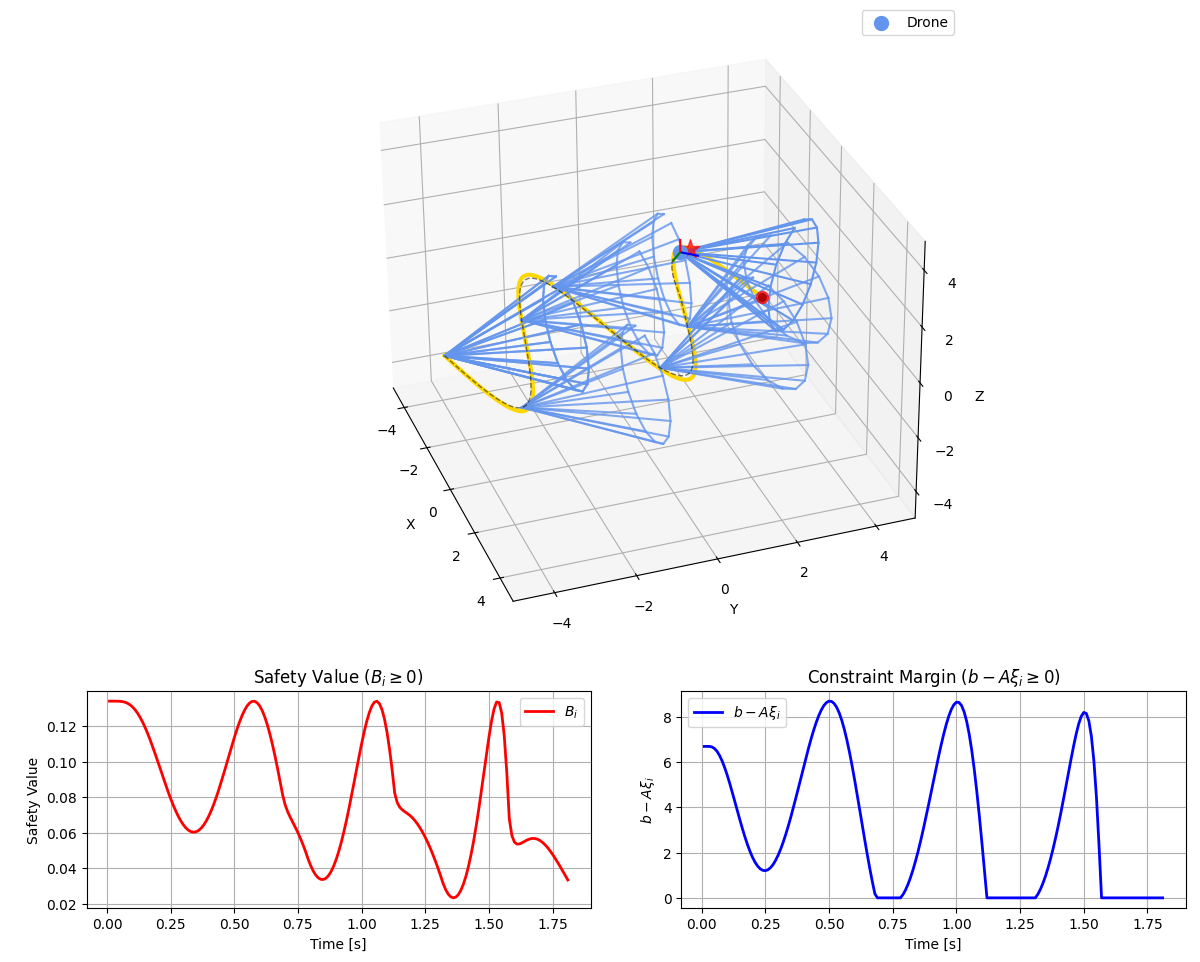
\includegraphics[width=0.6\linewidth]{fig/point_single.png}
\caption{単一特徴点追従におけるエージェントの軌跡と視野錐台}
\label{fig:single_trajectory}
\end{figure}

\subsection{単一エージェントにおける複数特徴点追従のためのCBF}

次に,単一エージェントが複数の特徴点を同時に追従する場合のシミュレーション結果について述べる.表\ref{tab:multi_point_params}に示すパラメータを用いてシミュレーションを実施した.ここで,前節のパラメータに加えて,$q$は\Eqref{eq:multi_safe_set}における確率制約パラメータである.

\begin{table}[htbp]
\centering
\caption{複数特徴点追従シミュレーションのパラメータ}
\label{tab:multi_point_params}
\begin{tabular}{cc}
\hline
変数名 & 値 \\
\hline
$h$ & $0.02$ \\
$\Psi_{\mathcal{F}}$ & $30^{\circ}$ \\
$Q_1$ & $\mathbf{I}_3$ \\
$Q_2$ & $0.0005\times\mathbf{I}_6$ \\
$q$ & $0.5$ \\
$\gamma_0$ & $5.0$ \\
\hline
\end{tabular}
\end{table}

図\ref{fig:multi_trajectory}に複数特徴点追従におけるエージェントの軌跡と視野錐台を示す.単一特徴点追従の場合と同様に,各タイムステップにおいてエージェント$i$が複数の特徴点を視野内に維持しながら追従していることが確認できる.安全制約$B_{i}$の値が常に正の値を保っており,CBFの正不変性が保証されていることがわかる.また,安全制約が減少傾向を示すタイムステップにおいて,制約余裕が零になっていることから,CBFが適切に機能していることが確認できる.

\begin{figure}[htbp]
\centering
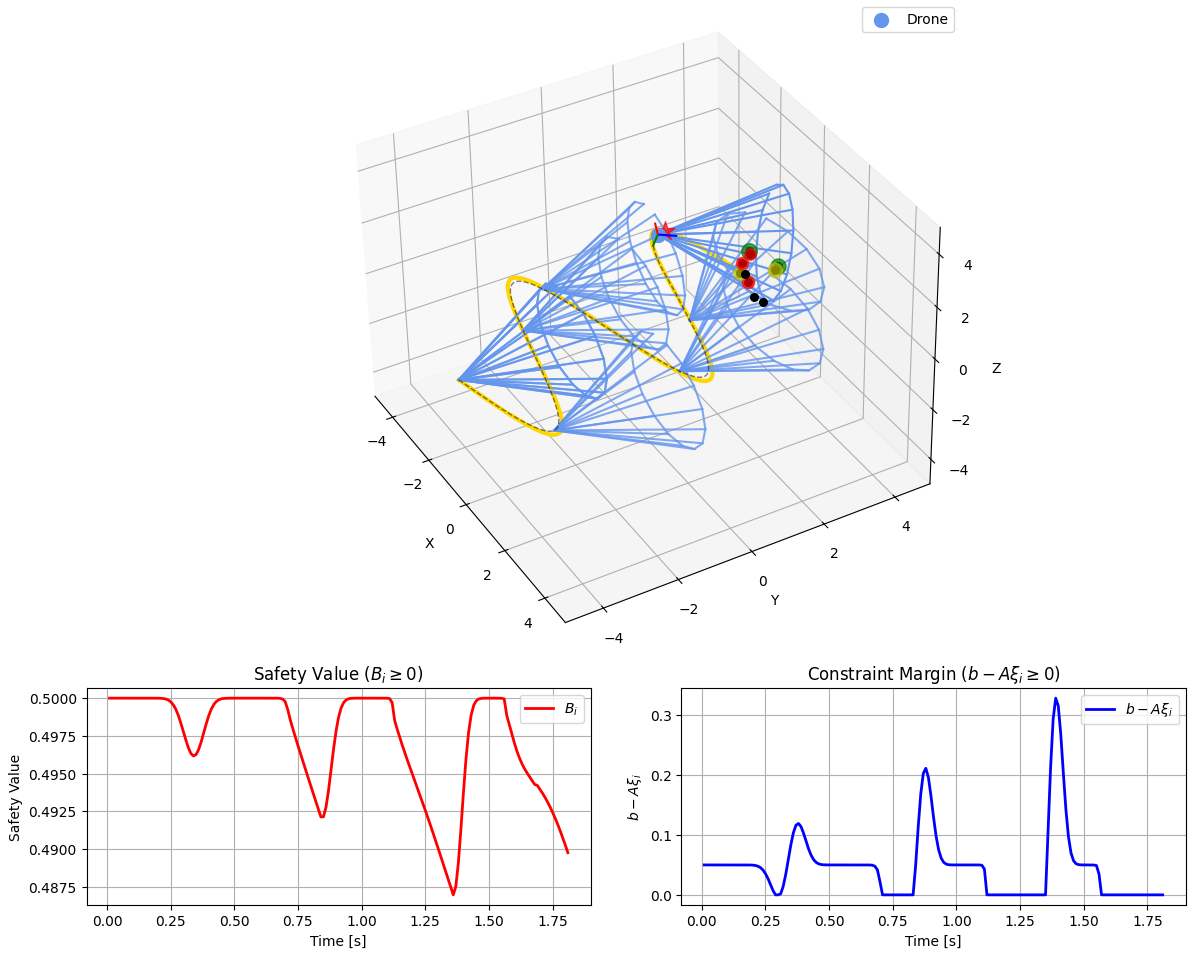
\includegraphics[width=0.6\linewidth]{fig/pcl_single.png}
\caption{複数特徴点追従におけるエージェントの軌跡と視野錐台}
\label{fig:multi_trajectory}
\end{figure}

\subsection{複数エージェントにおける複数特徴点追従のための集中型CBF}

続いて,複数エージェントが複数の特徴点を共有視野内に維持しながら追従する場合の集中型制御によるシミュレーション結果について述べる.表\ref{tab:centralized_params}に示すパラメータを用いてシミュレーションを実施した.

\begin{table}[htbp]
\centering
\caption{集中型制御シミュレーションのパラメータ}
\label{tab:centralized_params}
\begin{tabular}{cc}
\hline
変数名 & 値 \\
\hline
$h$ & $0.02$ \\
$\Psi_{\mathcal{F}}$ & $30^{\circ}$ \\
$Q_1$ & $\mathbf{I}_3$ \\
$Q_2$ & $0.0005\times\mathbf{I}_6$ \\
$q$ & $0.3$ \\
$\gamma_0$ & $0.1$ \\
\hline
\end{tabular}
\end{table}

図\ref{fig:centralized_trajectory}に集中型制御における複数エージェントの軌跡と視野錐台を示す.各タイムステップにおいて,エージェント$i$とエージェント$j$が共有特徴点を視野内に維持しながら協調して動作していることが確認できる.安全制約$B_{ij}$の値が常に正の値を保っており,CBFの正不変性が保証されていることがわかる.また,安全制約が減少傾向を示すタイムステップにおいて,制約余裕が零になっていることから,CBFが適切に機能していることが確認できる.

\begin{figure}[htbp]
\centering
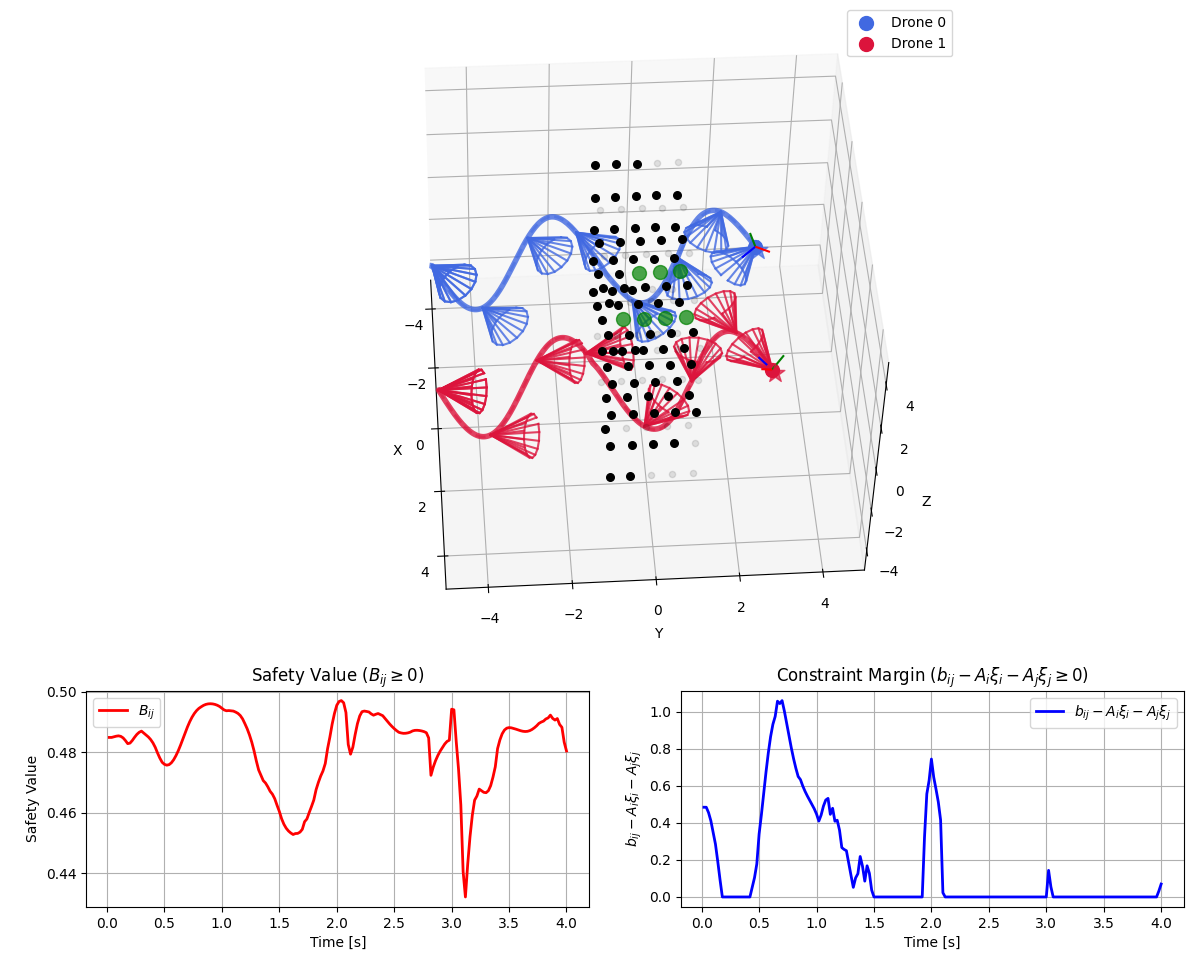
\includegraphics[width=0.6\linewidth]{fig/pcl_multi_centric.png}
\caption{複数特徴点追従における複数エージェントの軌跡と視野錐台}
\label{fig:centralized_trajectory}
\end{figure}

\subsection{複数エージェントにおける複数特徴点追従のための分散型CBF}

最後に,複数エージェントが複数の特徴点を共有視野内に維持しながら追従する場合の分散型制御によるシミュレーション結果について述べる.表\ref{tab:distributed_params}に示すパラメータを用いてシミュレーションを実施した.ここで,前節のパラメータに加えて,$c$は\Eqref{eq:pdmm_algorithm}における分散最適化のペナルティパラメータである.

\begin{table}[htbp]
\centering
\caption{分散型制御シミュレーションのパラメータ}
\label{tab:distributed_params}
\begin{tabular}{cc}
\hline
変数名 & 値 \\
\hline
$h$ & $0.02$ \\
$\Psi_{\mathcal{F}}$ & $30^{\circ}$ \\
$Q_1$ & $0.5\times \mathbf{I}_3$ \\
$Q_2$ & $0.00001\times\mathbf{I}_6$ \\
$q$ & $0.3$ \\
$\gamma_0$ & $0.1$ \\
$c$ & $1.0$ \\
\hline
\end{tabular}
\end{table}

図\ref{fig:distributed_trajectory}に分散型制御における複数エージェントの軌跡と視野錐台を示す.各タイムステップにおいて,エージェント$i$とエージェント$j$が共有特徴点を視野内に維持しながら協調して動作していることが確認できる.分散型最適化においては,元の制約式を直接解くことは不可能であるが,エージェント$i$が評価することのできる$A_i\xi_i-\frac{1}{2}b_{ij}$およびエージェント$j$の$A_j\xi_j-\frac{1}{2}b_{ij}$の和が適切に制約を満たしていることがわかる.これにより,各エージェントが局所的な情報のみを用いて,大域的な安全制約を満たす制御入力を生成できていることが確認できる.

\begin{figure}[htbp]
\centering
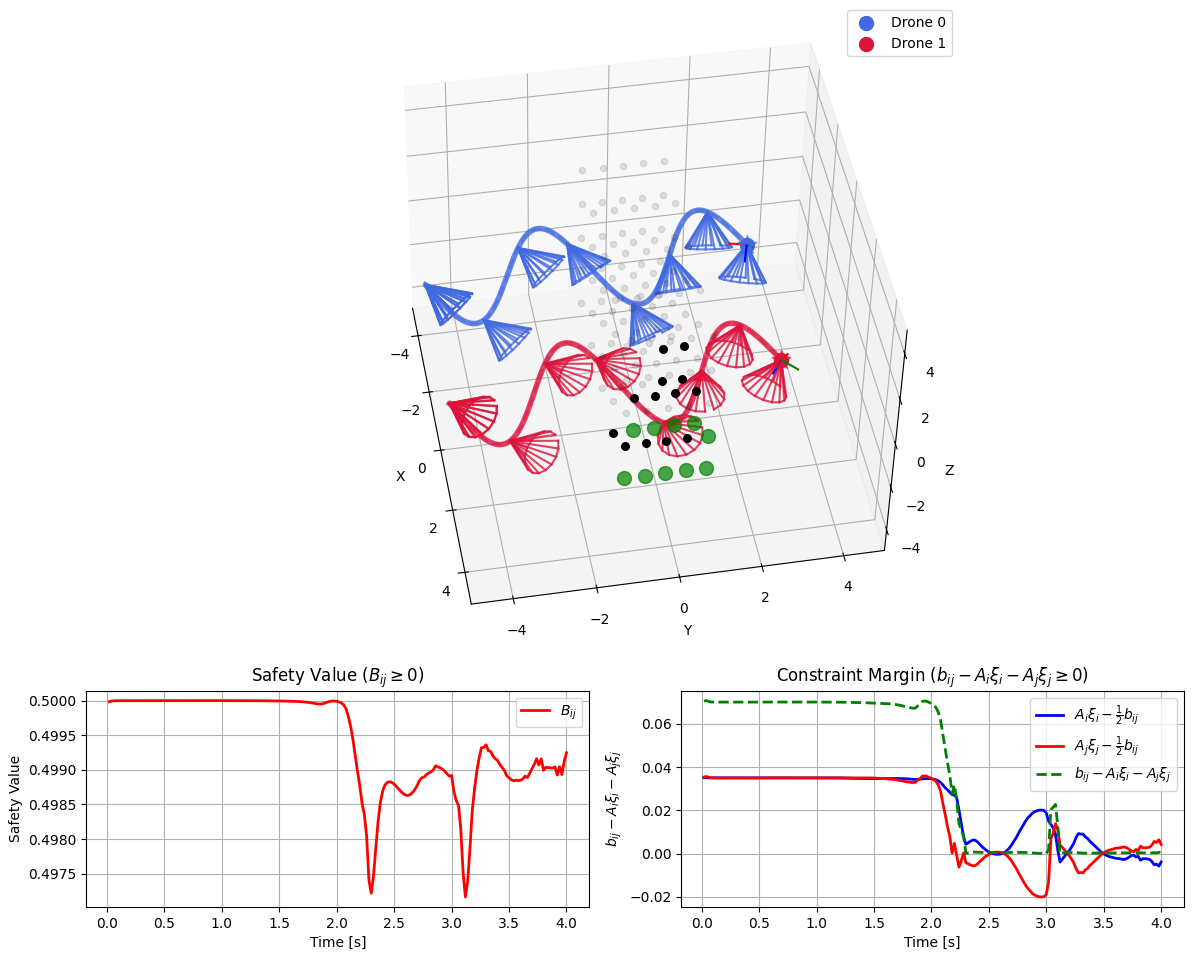
\includegraphics[width=0.6\linewidth]{fig/pcl_multi_distrib.png}
\caption{分散実装におけるエージェントの軌跡と視野錐台}
\label{fig:distributed_trajectory}
\end{figure}

以上のシミュレーション結果から,提案手法が単一エージェントおよび複数エージェントの両方において,特徴点を視野内に維持しながら追従するという制約を満たす制御入力を生成できることが確認された.特に,分散型実装においても,各エージェントが局所的な情報のみを用いて,大域的な安全制約を満たす制御入力を生成できることが示された.
